\begin{frame}{Preliminary on DQN \cite{DBLP:journals/corr/MnihKSGAWR13}}
\begin{enumerate}
    \item In contrast to TD-Gammon and similar approaches, a technique known as experience replay is used, where the agent’s experiences are stored at each time-step, $e_t = (s_t, a_t, r_t, s_{t+1})$ in a data-set $\mathcal{D} = e_1, \dots, e_N$ , pooled over many episodes into a replay memory.
    \item Q-learning updates, or minibatch updates are applied to samples of experience, $e \in \mathcal{D}$, drawn at random from the pool of stored samples.
    \begin{center}
        $L(\theta) = \mathbb{E}_{(s,a)}\Big[(y_j − Q(s , a ; \theta))^2\Big]$\\
        $\theta = \theta - \eta \nabla L(\theta)$
    \end{center}
    \item After performing experience replay, the agent selects and executes an action according to an $\epsilon$-greedy policy.
    \begin{center}
        With probability $\epsilon$ select a random action $a_t$\\
        otherwise select $a_t = \max_a Q(s_t, a; \theta)$
    \end{center}
    \item Learning from the randomized samples of experience replay memory reduces the correlations among samples and therefore reduces the variance of the updates.
\end{enumerate}
\end{frame}

\begin{frame}{DQN: Algorithm}
\begin{algorithm}[H]
\caption{Deep Q-learning with Experience Replay}
	\begin{algorithmic}[1]
	    \State Initialize replay memory $\mathcal{D}$ to capacity $N$;
	    \State Initialize action-value function $Q$ with random weights;
		\For {$episode=1,2,\ldots, M$}
		    \State Initialise sequence $s_1 = \{x_1\}$, preprocess sequence $\phi_1 = \phi(s_1)$
		    \For {$t=1,2,\ldots, T$} 
		    \State With probability $\epsilon$ select a random action $a_t$
		    \State otherwise select $a_t = \max_a Q(s_t, a; \theta)$ 
		    \State Execute action $a_t$ in emulator and observe reward $r_t$ and $x_{t+1}$
		    \State Set $s_{t+1} = s_t, a_t, x_{t+1}$ and preprocess $\phi_{t+1} = \phi(s_{t+1})$
		    \State Store transition $(\phi_t, a_t, r_t, \phi_{t+1})$ in $\mathcal{D}$
		    \State Sample random minibatch of transitions $(\phi_j , a_j , r_j , \phi_{j+1}) \in \mathcal{D}$
		    \State Set $y_j = \begin{cases}
		            r_j & for\, terminal \, \phi_{j+1} \\
		            r_j + \max_{a'} Q(\phi_{j+1}, a'; \theta) & for\, non-terminal \, \phi_{j+1}
		            \end{cases}$
		    \State Perform a gradient descent step on $(y_j − Q(\phi_j , a_j ; \theta))^2$
		    \EndFor
		\EndFor
	\end{algorithmic} 
\end{algorithm}
\end{frame}

\begin{frame}{Features}
\begin{enumerate}
    \item \textbf{News features} describe whether certain property appears in this piece of news, including headline, provider, ranking, entity name, category, topic category, and click counts in last 1 hour, 6 hours, 24 hours, 1 week, and 1 year respectively.
    \item \textbf{User features} mainly describes the features (i.e., headline, provider, ranking, entity name, category, and topic category) of the news that the user clicked in 1 hour, 6 hours, 24 hours, 1 week, and 1 year respectively.
    \item \textbf{User news features} describe the interaction between user and one certain piece of news, i.e., the frequency for the entity (also category, topic category and provider) to appear in the history of the user’s readings.
    \item \textbf{Context features} describe the context when a news request happens, including time, weekday, and the freshness of the news (the gap between request time and news publish time).
\end{enumerate}
    
\end{frame}

\begin{frame}{DRN Framework \cite{10.1145/3178876.3185994}}
\begin{enumerate}
    \item The total reward is modeled as follows:
    \begin{center}
        $y_{(s,a)} = Q(s, a) = r_{immediate} + \gamma r_{future}$.    
    \end{center}
    where $r_{immediate}$ represents the rewards (e.g., whether user click on this piece of news) for current situation, and $r_{future}$ represents the agent’s projection of future rewards.
    
    \item In this formulation, agent G will speculate the next state $s_{a,t+1}$, given action $a$ is selected. Based on this, given a candidate set of actions {$a'$}, the action $a'$ that gives the maximum future reward is selected according to parameter $W_t$. After this, the estimated future reward given state $s_{a,t+1}$ is calculated based on $W′_t$.
    \begin{center}
        $y_{s,a,t} = r_{a,t+1} + \gamma Q(s_{a,t+1}, \argmax\limits_{a'} Q(s_{a,t+1}, a'; W_t ); W'_t)$
    \end{center}
    Here, $W_t$ and $W'_t$ are two different sets of parameters of the DQN
    
    \item User features and Context features are used as state features, while User news features and Context features are used as action features.
    
\end{enumerate}
\end{frame}

\begin{frame}{Model Framework}
        \begin{figure}
            \centering
            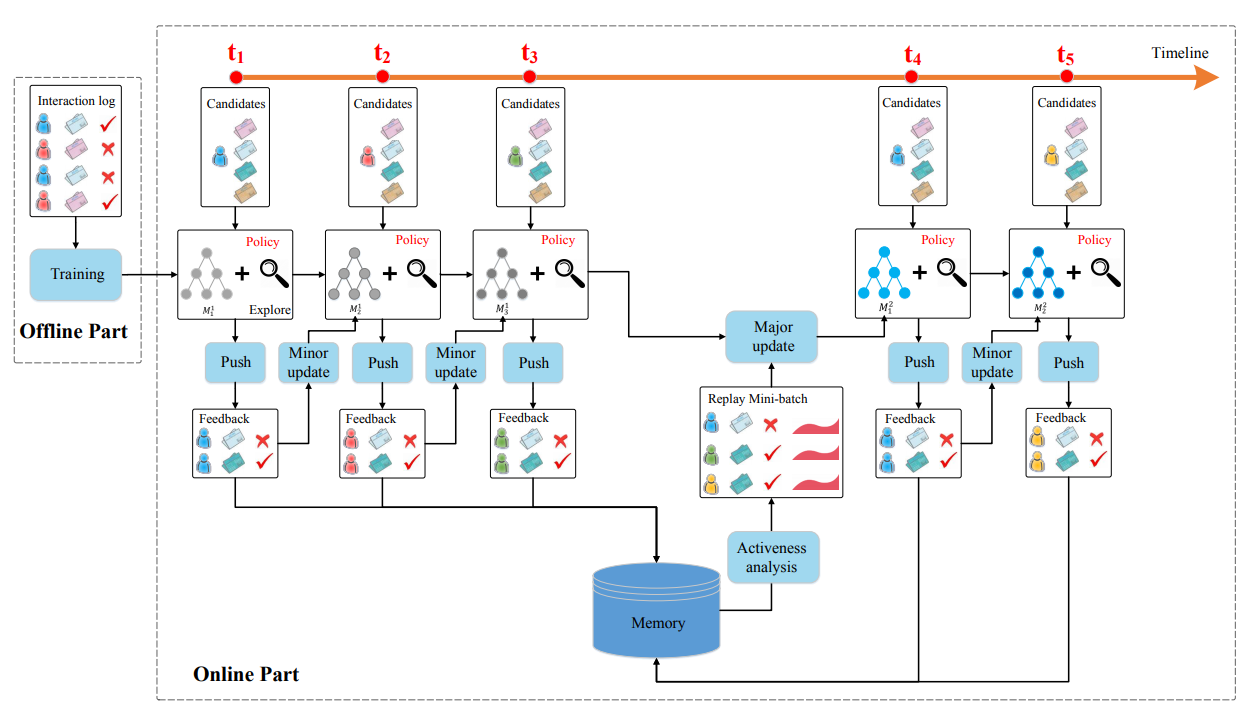
\includegraphics[scale = 0.25]{PPT/model_framework.png}
            \caption{Model Framework}
        \end{figure}
\end{frame}